\documentclass[14pt]{extbook}
\usepackage{multicol, enumerate, enumitem, hyperref, color, soul, setspace, parskip, fancyhdr} %General Packages
\usepackage{amssymb, amsthm, amsmath, bbm, latexsym, units, mathtools} %Math Packages
\everymath{\displaystyle} %All math in Display Style
% Packages with additional options
\usepackage[headsep=0.5cm,headheight=12pt, left=1 in,right= 1 in,top= 1 in,bottom= 1 in]{geometry}
\usepackage[usenames,dvipsnames]{xcolor}
\usepackage{dashrule}  % Package to use the command below to create lines between items
\newcommand{\litem}[1]{\item#1\hspace*{-1cm}\rule{\textwidth}{0.4pt}}
\pagestyle{fancy}
\lhead{Makeup Progress Quiz 3}
\chead{}
\rhead{Version C}
\lfoot{4315-3397}
\cfoot{}
\rfoot{Fall 2020}
\begin{document}

\begin{enumerate}
\litem{
Evaluate the one-sided limit of the function $f(x)$ below, if possible.\[ \lim_{x \rightarrow -8^-} \frac{6}{(x-8)^6}+5 \]\begin{enumerate}[label=\Alph*.]
\item \( f(-8) \)
\item \( -\infty \)
\item \( \infty \)
\item \( \text{The limit does not exist} \)
\item \( \text{None of the above} \)

\end{enumerate} }
\litem{
For the graph below, evaluate the limit: $ \displaystyle \lim_{x \rightarrow -4} f(x)$.
\begin{center}
    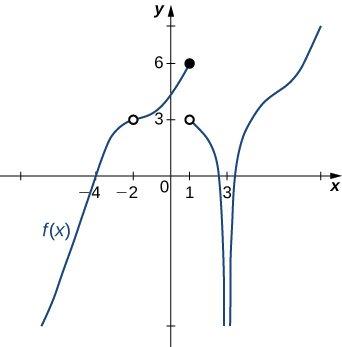
\includegraphics[width=0.5\textwidth]{../Figures/evaluateLimitGraphicallyC.png}
\end{center}
\begin{enumerate}[label=\Alph*.]
\item \( -\infty \)
\item \( -6 \)
\item \( 0 \)
\item \( \text{The limit does not exist} \)
\item \( \text{None of the above} \)

\end{enumerate} }
\litem{
To estimate the one-sided limit of the function below as $x$ approaches 4 from the left, which of the following sets of numbers should you use?\[ \frac{\frac{4}{x} - 1}{x - 4} \]\begin{enumerate}[label=\Alph*.]
\item \( \{ 3.9000, 3.9900, 3.9990, 3.9999 \} \)
\item \( \{ 4.0000, 3.9000, 3.9900, 3.9990 \} \)
\item \( \{ 4.1000, 4.0100, 4.0010, 4.0001 \} \)
\item \( \{ 3.9000, 3.9900, 4.0100, 4.1000 \} \)
\item \( \{ 4.0000, 4.1000, 4.0100, 4.0010 \} \)

\end{enumerate} }
\litem{
Based on the information below, which of the following statements is always true?
\begin{center}
    \textit{ $f(x)$ approaches $3.476$ as $x$ approaches $1$. }
\end{center}
\begin{enumerate}[label=\Alph*.]
\item \( f(1) \text{ is close to or exactly } 3 \)
\item \( f(3) \text{ is close to or exactly } 1 \)
\item \( f(3) = 1 \)
\item \( f(1) = 3 \)
\item \( \text{None of the above are always true.} \)

\end{enumerate} }
\litem{
For the graph below, evaluate the limit: $ \displaystyle \lim_{x \rightarrow 1} f(x)$.
\begin{center}
    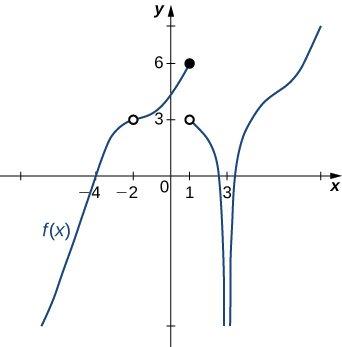
\includegraphics[width=0.5\textwidth]{../Figures/evaluateLimitGraphicallyCopyC.png}
\end{center}
\begin{enumerate}[label=\Alph*.]
\item \( 3 \)
\item \( 6 \)
\item \( -\infty \)
\item \( \text{The limit does not exist} \)
\item \( \text{None of the above} \)

\end{enumerate} }
\litem{
Evaluate the one-sided limit of the function $f(x)$ below, if possible.\[ \lim_{x \rightarrow 4^+} \frac{7}{(x-4)^9}+9 \]\begin{enumerate}[label=\Alph*.]
\item \( -\infty \)
\item \( f(4) \)
\item \( \infty \)
\item \( \text{The limit does not exist} \)
\item \( \text{None of the above} \)

\end{enumerate} }
\litem{
To estimate the one-sided limit of the function below as $x$ approaches 3 from the right, which of the following sets of numbers should you use?\[ \frac{\frac{3}{x} - 1}{x - 3} \]\begin{enumerate}[label=\Alph*.]
\item \( \{ 3.0000, 2.9000, 2.9900, 2.9990 \} \)
\item \( \{ 3.1000, 3.0100, 3.0010, 3.0001 \} \)
\item \( \{ 2.9000, 2.9900, 2.9990, 2.9999 \} \)
\item \( \{ 2.9000, 2.9900, 3.0100, 3.1000 \} \)
\item \( \{ 3.0000, 3.1000, 3.0100, 3.0010 \} \)

\end{enumerate} }
\litem{
Based on the information below, which of the following statements is always true?
\begin{center}
    \textit{ $f(x)$ approaches $7.145$ as $x$ approaches $2$. }
\end{center}
\begin{enumerate}[label=\Alph*.]
\item \( f(x) = 2 \text{ when } x \text{ is close to } 7.145 \)
\item \( f(x) = 7.145 \text{ when } x \text{ is close to } 2 \)
\item \( f(x) \text{ is close to or exactly } 7.145 \text{ when } x \text{ is close to } 2 \)
\item \( f(x) \text{ is close to or exactly } 2 \text{ when } x \text{ is close to } 7.145 \)
\item \( \text{None of the above are always true.} \)

\end{enumerate} }
\litem{
Evaluate the limit below, if possible.\[ \lim_{x \rightarrow 8} \frac{\sqrt{9x - 23} - 7}{7x - 56} \]\begin{enumerate}[label=\Alph*.]
\item \( 0.429 \)
\item \( \infty \)
\item \( 0.010 \)
\item \( 0.071 \)
\item \( \text{None of the above} \)

\end{enumerate} }
\litem{
Evaluate the limit below, if possible.\[ \lim_{x \rightarrow 7} \frac{\sqrt{4x - 12} - 4}{9x - 63} \]\begin{enumerate}[label=\Alph*.]
\item \( 0.014 \)
\item \( 0.125 \)
\item \( 0.056 \)
\item \( \infty \)
\item \( \text{None of the above} \)

\end{enumerate} }
\end{enumerate}

\end{document}